
\newif\ifshowsolutions
\showsolutionstrue
\documentclass{article}
\usepackage{listings}
\usepackage{amsmath}
%\usepackage{subfigure}
\usepackage{subfig}
\usepackage{amsthm}
\usepackage{amsmath}
\usepackage{amssymb}
\usepackage{graphicx}
\usepackage{mdwlist}
\usepackage[colorlinks=true]{hyperref}
\usepackage{geometry}
\usepackage{titlesec}
\geometry{margin=1in}
\geometry{headheight=2in}
\geometry{top=2in}
\usepackage{palatino}
\usepackage{mathrsfs}
\usepackage{fancyhdr}
\usepackage{paralist}
\usepackage{todonotes}
\setlength{\marginparwidth}{2.15cm}
\usepackage{tikz}
\usetikzlibrary{positioning,shapes,backgrounds}
\usepackage{float} % Place figures where you ACTUALLY want it
\usepackage{comment} % a hack to toggle sections
\usepackage{ifthen}
\usepackage{mdframed}
\usepackage{verbatim}
\usepackage[strings]{underscore}
\usepackage{listings}
\usepackage{bbm}
\rhead{}
\lhead{}

\renewcommand{\baselinestretch}{1.15}

% Shortcuts for commonly used operators
\newcommand{\E}{\mathbb{E}}
\newcommand{\Var}{\operatorname{Var}}
\newcommand{\Cov}{\operatorname{Cov}}
\newcommand{\Bias}{\operatorname{Bias}}
\DeclareMathOperator{\argmin}{arg\,min}
\DeclareMathOperator{\argmax}{arg\,max}

% do not number subsection and below
\setcounter{secnumdepth}{1}

% custom format subsection
\titleformat*{\subsection}{\large\bfseries}

% set up the \question shortcut
\newcounter{question}[section]
\newenvironment{question}[1][]
  {\refstepcounter{question}\par\addvspace{1em}\textbf{Question~\Alph{question}\!
    \ifthenelse{\equal{#1}{}}{}{ [#1 points]}: }}
    {\par\vspace{\baselineskip}}

\newcounter{subquestion}[question]
\newenvironment{subquestion}[1][]
  {\refstepcounter{subquestion}\par\medskip\textbf{\roman{subquestion}.\!
    \ifthenelse{\equal{#1}{}}{}{ [#1 points]:}} }
  {\par\addvspace{\baselineskip}}

\titlespacing\section{0pt}{12pt plus 2pt minus 2pt}{0pt plus 2pt minus 2pt}
\titlespacing\subsection{0pt}{12pt plus 4pt minus 2pt}{0pt plus 2pt minus 2pt}
\titlespacing\subsubsection{0pt}{12pt plus 4pt minus 2pt}{0pt plus 2pt minus 2pt}


\newenvironment{hint}[1][]
  {\begin{em}\textbf{Hint: }}{\end{em}}

\ifshowsolutions
  \newenvironment{solution}[1][]
    {\par\medskip \begin{mdframed}\textbf{Solution~\Alph{question}#1:} \begin{em}}
    {\end{em}\medskip\end{mdframed}\medskip}
  \newenvironment{subsolution}[1][]
    {\par\medskip \begin{mdframed}\textbf{Solution~\Alph{question}#1.\roman{subquestion}:} \begin{em}}
    {\end{em}\medskip\end{mdframed}\medskip}
\else
  \excludecomment{solution}
  \excludecomment{subsolution}
\fi
\newcommand{\boldline}[1]{\underline{\textbf{#1}}}

\usepackage{graphicx}
\graphicspath{ {images/} }

\chead{%
  {\vbox{%
      \vspace{2mm}
      \large
      Machine Learning \& Data Mining \hfill
      Caltech CS/CNS/EE 155 \hfill \\[1pt]
      Miniproject 3\hfill
      Released March $3^{rd}$, 2017 \\
    }
  }
}

\begin{document}
\pagestyle{fancy}

% LaTeX is simple if you have a good template to work with! To use this document, simply fill in your text where we have indicated. To write mathematical notation in a fancy style, just write the notation inside enclosing $dollar signs$.

% For example:
% $y = x^2 + 2x + 1$

% For help with LaTeX, please feel free to see a TA!

%%%%%%%%%%%%%%%%%%%%%%%%%%%%%%%%%%%%%%%%%%%%%%%%%%%%%%%%%%%%%%%%%%%%%%%%%%%%%%%%%%%%%%%%

\section{Introduction}
\medskip
\begin{itemize}
    \item \textbf{Group members:} Enrico Borba, Claire Goeckner-Wald
    \item \textbf{Team name:} Papa Mart's Mini Gary - The End
    \item \textbf{Division of labour:}
        Enrico Borba: Programming, ideas, report visualization.
        Claire Goeckner-Wald: Programming, ideas, report assembly.
\end{itemize}


%%%%%%%%%%%%%%%%%%%%%%%%%%%%%%%%%%%%%%%%%%%%%%%%%%%%%%%%%%%%%%%%%%%%%%%%%%%%%%%%%%%%%%%%
\section{Basic Visualizations}
\medskip
% - Justify your choice of visualization method
% - What did you observe?
% - Did the results match what you would expect to see?
% - How do the ratings of the best movies compare to those of those of the most popular movies
% - How do the ratings of the three genres you chose compare to one another
% - Any other comparisons/observations

\begin{itemize}
  \item \textbf{Choice of visualization method:} We used a line graph to show visualize the dataset. We didn't use histograms, because the amount of data shown on the chart would have overwhelmed the reader using this method. For visualizing our three genres, we used the size of the dot to indicate the number of genres the movie is in (larger dot implies more genre crossover); the color of the dot indicated the standard deviation of the reviews (yellow implies higher standard deviation, blue implies lower standard deviation.)
  \item \textbf{Observations:} We observed that 3 was not the average rating, perhaps unsurprisingly. While one might expect a uniform, or normal distribution, center around 3 stars, 4 stars was in fact the most common rating given. On second thought, this is perhaps more expected, because people will tend to watch movies they enjoy - so that would skew the distribution towards higher ratings.
  \begin{center}
    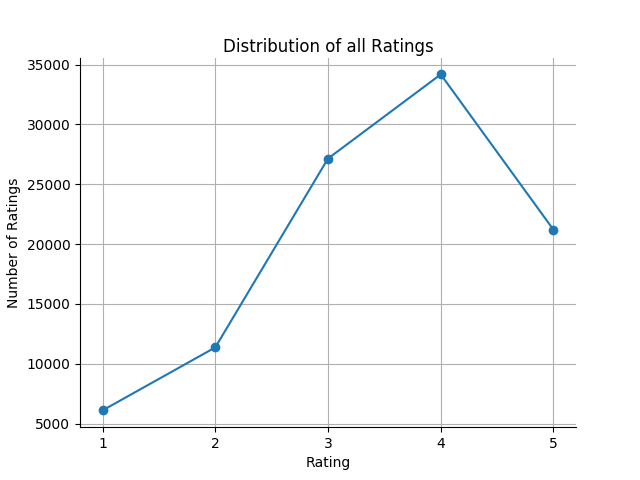
\includegraphics[scale=.6]{basic_1.png}
  \end{center}
  \item \textbf{Results:} The results approximately matched what we expected.
  \item \textbf{Best ratings:} With the exception of Star Wars, none of the top 10 movies with the highest number of ratings overlapped with the top 10 highest average-rated movies. This is perhaps unexpected. To visualize the highest average-rating movies, we decided to use the size of the line to indicate the number of ratings for the film. This visualization method really shows how much Star Wars stands out. In order to acquire this list, we did not include films with fewer than 50 ratings, which removed 
  \begin{center}
    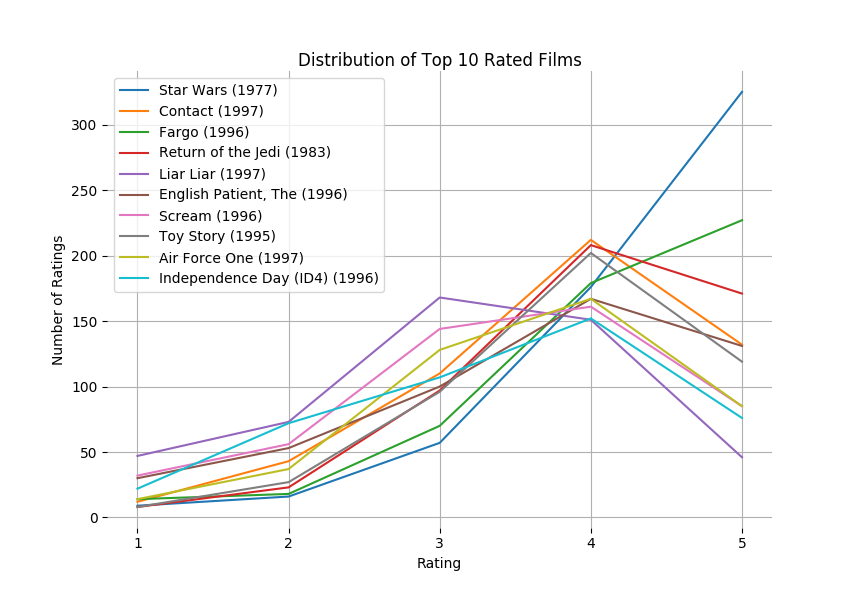
\includegraphics[scale=.5]{basic_2.png} \\
    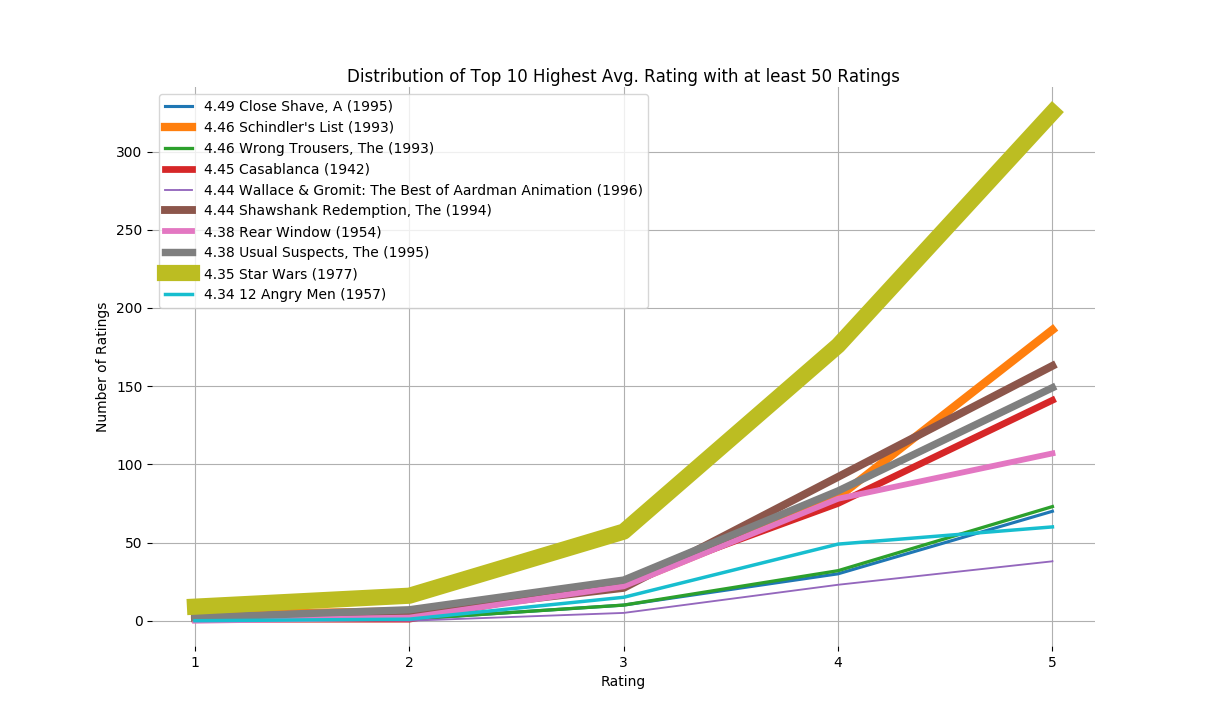
\includegraphics[scale=.4]{basic_3.png}
  \end{center}
  \item \textbf{Three genres:} We note that the SciFi genre has no movies rated over 4 stars with less than about 200 ratings. We postulate that this is because SciFi's are more difficult to produce, and thus the better scifi films (those with funding) would correlate with more/better advertising (and thus more ratings). As a reminder, we used the size of the dot to indicate the number of genres the movie is in (larger dot implies more genre crossover); the color of the dot indicated the standard deviation of the reviews (yellow implies higher standard deviation, blue implies lower standard deviation.)
  \begin{center}
    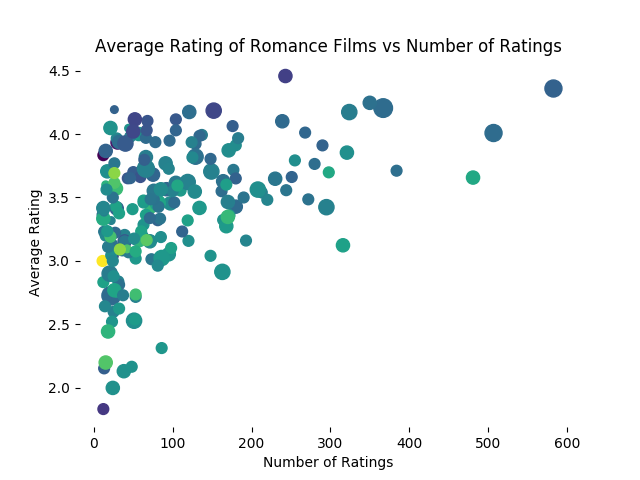
\includegraphics[scale=.3]{basic_4_romance.png} 
    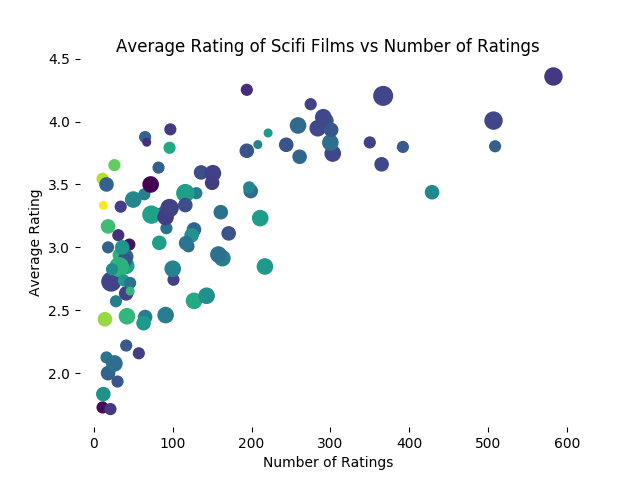
\includegraphics[scale=.3]{basic_4_scifi.png}
    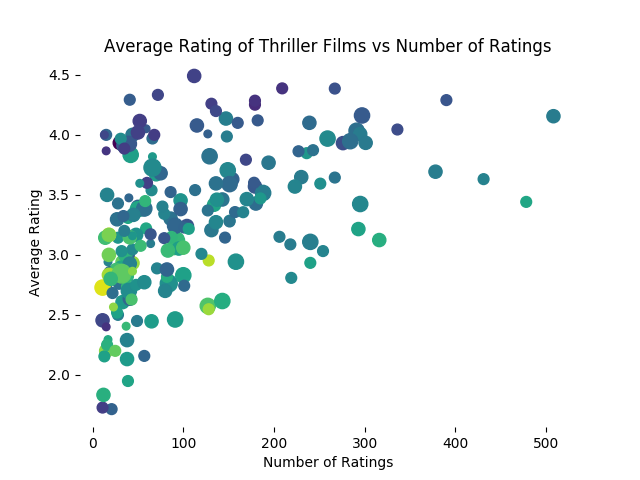
\includegraphics[scale=.3]{basic_4_thriller.png}
  \end{center}
\end{itemize}


%%%%%%%%%%%%%%%%%%%%%%%%%%%%%%%%%%%%%%%%%%%%%%%%%%%%%%%%%%%%%%%%%%%%%%%%%%%%%%%%%%%%%%%%
\section{Matrix Factorization Algorithm}
\medskip
% - What parameters did you adjust and how?
% - Justify your choices for the parameters and stopping criteria
% - Did you make any other significant modifications or additions
\begin{itemize}
  \item \textbf{Adjustment of parameters:}
  \item \textbf{Justification of parameters and stopping criteria:}
  \item \textbf{Significant modifications:}
\end{itemize}


%%%%%%%%%%%%%%%%%%%%%%%%%%%%%%%%%%%%%%%%%%%%%%%%%%%%%%%%%%%%%%%%%%%%%%%%%%%%%%%%%%%%%%%%
\section{Marix Factorization Visualization}
\medskip
% - What did you observe?
% - How do the visualizations of the best movies compare to those of the most popular movies
% - How do the visualizations of the three genres you chose compare to one another
% - What was expected and what was surprising from the visualizations?
% - Any other comparisons/observations
\begin{itemize}
  \item \textbf{Observations:} We observed that the matrix factorization method revealed unexpected relationships between some movies. 
  \item \textbf{Best/most ratings:} In the top 10 most rated films, there is a marked clustering of 8 of the 10 movies - \textit{Return of the Jedi} and \textit{Contact} are outliers. The distance of \textit{Return of the Jedi} may not be unexpected, due to the remarkable popularity and high ratings that the Star Wars franchise has enjoyed, in general. \textit{Contact} is a 1997 science fiction drama film based on the writings of Carl Sagan. In retrospect, it might be better to plot the two following graphs on the same chart, to tell us more about their respective positions. Either that, or fix the axis. 
  \begin{center}
    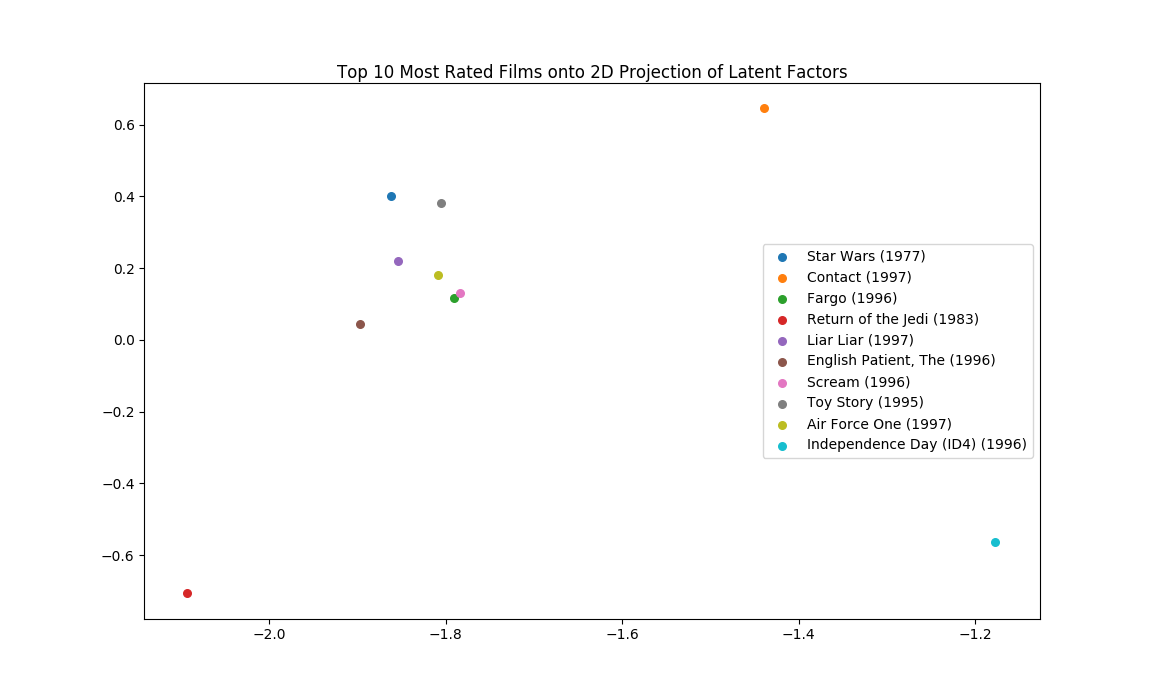
\includegraphics[scale=.45]{mat_fac_2.png}
    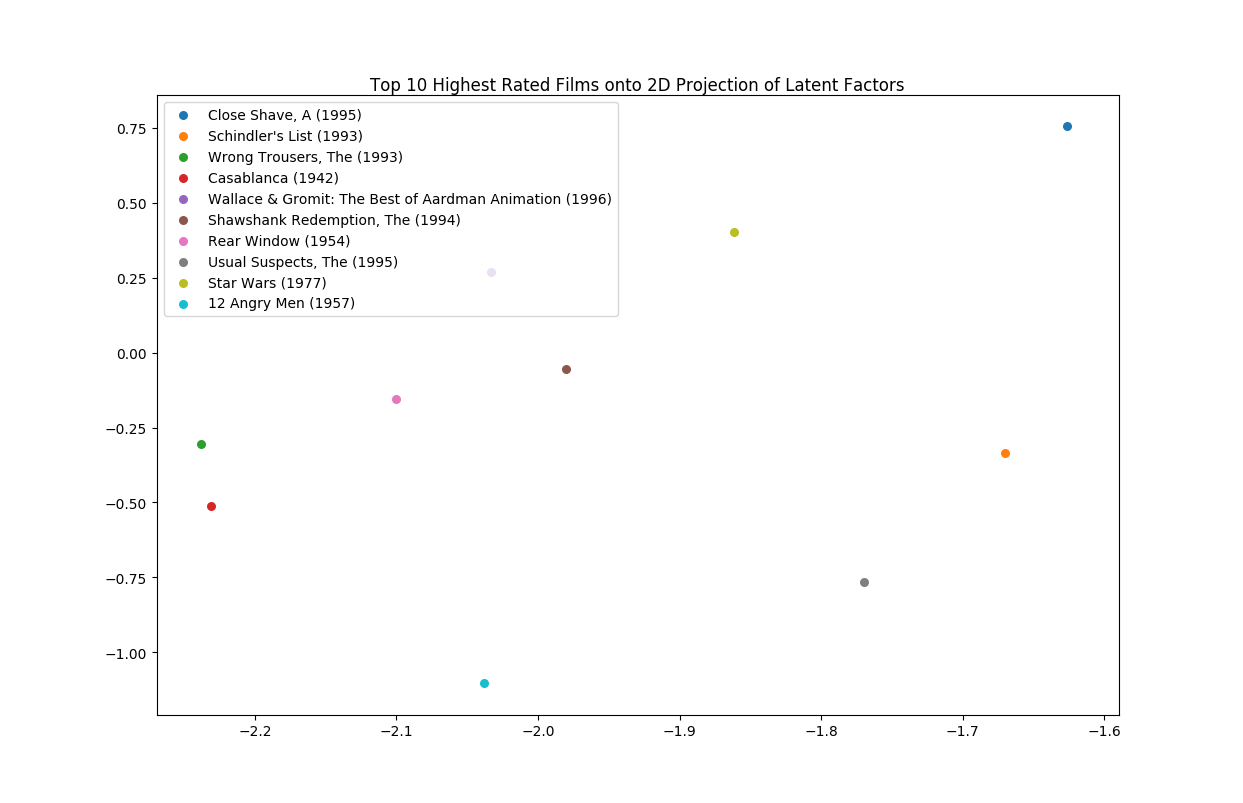
\includegraphics[scale=.45]{mat_fac_3.png}
  \end{center}
  \item \textbf{Three genres:} We sampled films from Romance, SciFi, and Thriller. There appears to be some mild to moderate clustering of points, but the films are overall hard to distinguish from location alone, by human eye.
  \begin{center}
    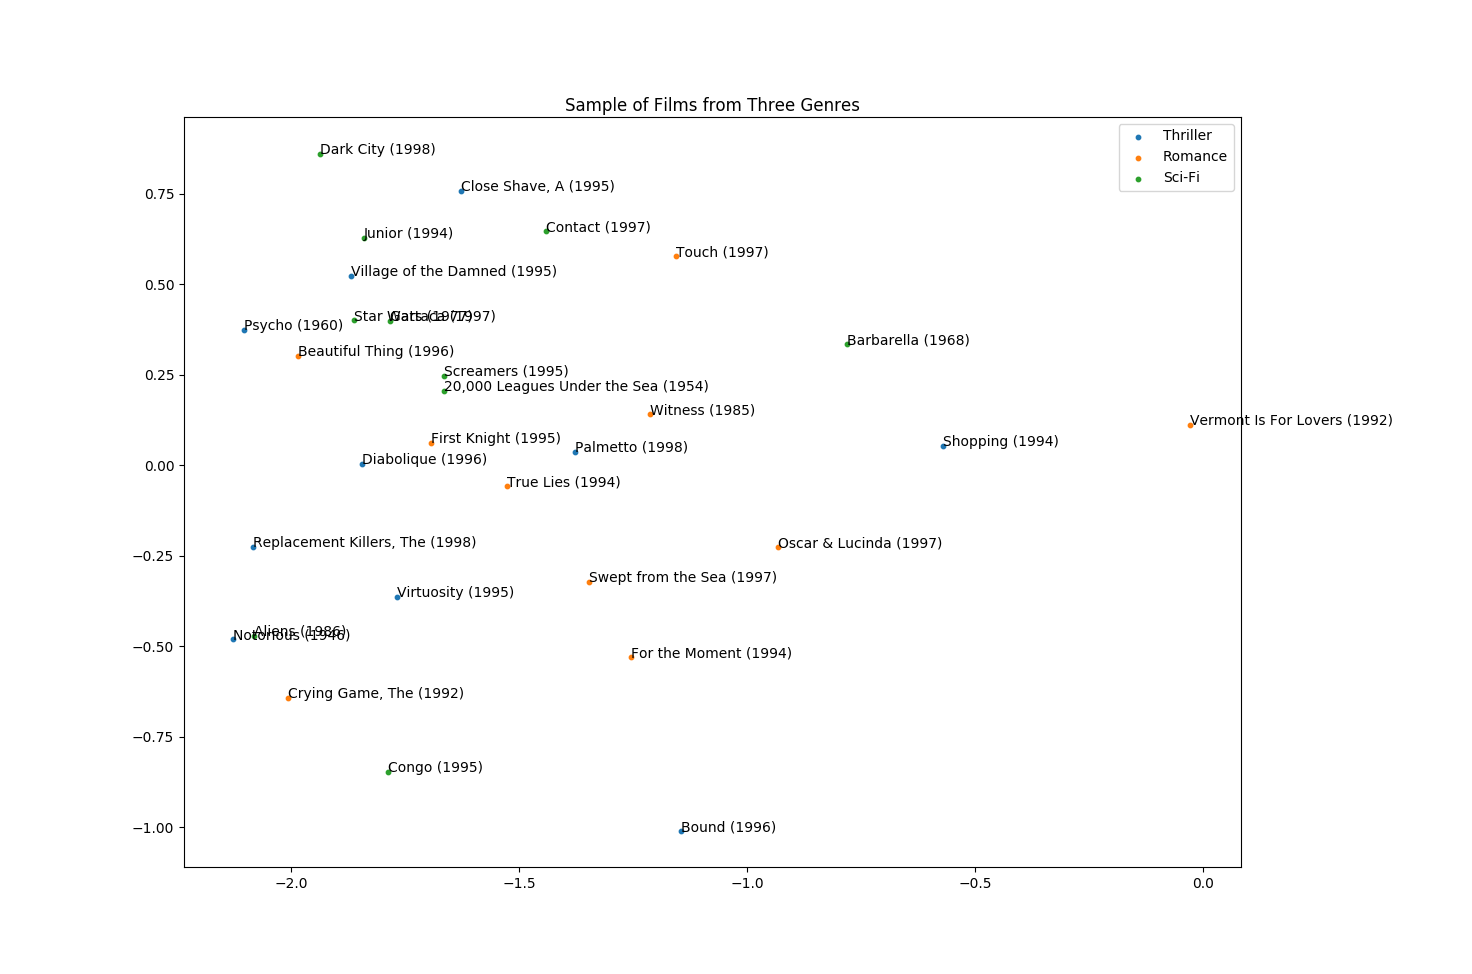
\includegraphics[scale=.45]{mat_fac_4.png}
  \end{center}
  \item \textbf{Expected, and unexpected:} We expected more demonstrable clustering of points in the three genres. We also noticed that \textit{Gattaca} and \textit{Star Wars} were very, very close together, as well as a handful of other movie pairings. We guess that this makes a statement on the similarities of the movies. However, this one makes more sense than some other film pairings. Some pairs are:
  \begin{itemize}
    \item \textit{Gattaca} and \textit{Star Wars} (A 1997 science fiction biopunk and a 1977 space opera epic)
    \item \textit{Screamers} and \textit{20,000 Leagues Under the Sea} (A 1995 dystopian science fiction and a 1954 Technicolor science fiction)
    \item \textit{Aliens} and \textit{Notorious} (A 1986 science fiction action horror and a 200biographical drama about Notorious B.I.G.)
  \end{itemize}
  Weirdly, all of the above are SciFi, with the exception of Notorious, which was a Thriller.
\end{itemize}



%%%%%%%%%%%%%%%%%%%%%%%%%%%%%%%%%%%%%%%%%%%%%%%%%%%%%%%%%%%%%%%%%%%%%%%%%%%%%%%%%%%%%%%%
\section{Conclusions}
\medskip
% - Briefly summarize your main observations
% - Did your visualizations help you to better understand the MovieLens dataset?
\begin{itemize}
  \item \textbf{Summary:} Our main observations were that `top-rated' and `best-rated' movies tend to be two very different things. Moreover, the matrix factorization revealed unusual relationships between certain movies. 
  \item \textbf{Did it help?:} The visualizations helped us better understand the MovieLens dataset. 
\end{itemize}


\end{document}